\chapter{Introduction}
\label{ch:Intro}


%%%%%%%%%%%%%%%%%%%%%%%%%%%%%%%%%%%%%%%%%%%%%%%%%%


\section{Psoriasis and psoriatic arthritis}
%
Psoriasis and psoriatic arthritis (PsA) have been progressively identified as two different common complex disease entities. Psoriasis is a chronic inflammatory dermatose disease with episodes of relapse and remitance \parencite{Nestle2009}. On the other hand, PsA is a seronegative chronic inflammatory disease within the family of spondyloarthritis \parencite{Moll1973, Coates2016} that usually develops after the psoriasis skin manifestations\parencite{Villanova2016}. Psoriasis and PsA have shared and distinct clinical features, which are likely a reflection of the commonalities and differences in genetic loci contributing to disease development. It is important to understand those commonalities and differences at the physiological and genetic level in order to better understand the relevance of the genetic variability in the risk to develop psoriasis and PsA.

%(Variants in RUNX3 contribute to susceptibility to PsA, exhibiting further common ground with ankylosing spondylitis, PsA Immunochip)

\subsection{Epidemiology and global impact}
%
Psoriasis represents a serious global health problem that currently affects about 100 million people worldwide, including children and adults with no sex bias \parencite{Organization2016}. Although there is a very weak correlation with geographic latitude \parencite{Jacobson2011}, it has been reported to vary upon ethnicity. For example, psoriasis prevalence in adults is lower among African, African American and Asian (0.4-0.7\%) compared to American and Canadian (4.6 and 4.7\%, respectively) populations. In the UK, psoriasis prevalence ranges between 2-3\% and it affects approximately 1.8 million people \parencite{Perera2012}.

PsA prevalence in the general population ranges between 0.04-1.2\% \parencite{Perera2012}but it dramatically increases to 10-30\% within psoriasis cases \parencite{Gelfand2005,Reich2008} and evidences the association between the two diseases. Particularly, in the UK, 14\% of the psoriasis patients develop chronic inflammatory arthritis in the form of PsA at some point of the disease course \parencite{Ibrahim2009}. %Overall, data suggests an steady increase in both, psoriasis and PsA, prevalence over time \parencite{Springate2007,Organization2016}.

Although psoriasis can be developed at any age, onset of disease seems to have a bimodal distribution strongly influenced by the Human Leukocyte Antigen (HLA) Cw*06:02 (HLA-Cw6:02), an allele for one of the genes in the Major Histocompatibility Complex (MHC), involved in antigen presentation \parencite{Henseler1985} and the strongest genetic association with psoriasis and PsA risk \parencite(Ellinghaus2010, Strange2010, Stuart2010; Sun2010). The early-onset or Type I is characterised by development of disease around 16-22 and 30-39 years and a prevalence for HLA-C*06:02 (85.4\% of the cases). In contrasts, the late-onset or Type II group manifests disease between 50-60 years old and presents positive HLA-C*06:02 only in 14.6\% of the cases. %This classification based on the age of onset has also correlates with distinctive clinical clinical features including severity, relapse frequency and family history.

Psoriasis and PsA also represent an economical burden for the countries' economies due to treatment and associated morbidity. For example, in the UK treatment and management of psoriasis in 2015 ranged between £4,000 to £14,000, before and after requirements of biological therapy, respectively \parencite{Burgos-Pol2016} and the costs are even greater for PsA \parencite{Poole2010}.


\subsection{Psoriasis and inflammatory dermatoses}
%

The group of inflammatory dermatoses affects up to 70\% of the population, regardless age and geographic location \parencite{ICD-10}, and it represents the 4$^{th}$ leading cause of nonfatal burden \parencite{Roderick2014}. The skin is the biggest organ in the human body constituting an effective barrier between the environment and the internal organs. The most external layer, the epidermis, plays a relevant role in the innate and adaptive immunity \parencite{Proksch2008} and its alterations due to exogenous or endogenous factors can lead to development of inflammatory dermatose conditions, such as psoriasis, atopic dermatitis (AD) or cutaneous lupus erythematosus (CLE) \parencite{Johnson-Huang,2009}. Lesions in psoriasis can be non-pustular and pustular which reflects the heterogeneity in the type, location and severity of the disease and impairs the clinical classification \parencite{Perera2012}. As a result, several phenotypes of psoriasis including vulgaris, guttate, pustular, erythroderma and nail pitting have been defined and it is under debate whether some of those should be considered a different disease entity \parencite{Marrakchi2011}.


\subsection{PsA and spondyloarthropaties}
%
PsA belong to the family known as spondylarthropaties (SpA) which also includes other subtypes such as ankylosing spondylitis (AS), reactive arthritis (ReA), idiopathic inflammatory bowel disease (IBD) and undifferentiated SpA \parencite{Baeten2013}. All SpA subtypes are characterised by structural damage (bone formation and erosion) as well as inflammation of joints and extraarticular sites such as eyes, gut and skin. Additional SpA criteria have led to a reduced classification of SpA into axial and peripheral SpA based on the affected joint (spine/sacroilicac or peripheral) and the presence of extraarticular features \parencite{Runwaleit2001, Runwaleit2001}. Studies in human families and rat models with HLA-B27 positive status have shown manifestation of different SpA forms, such as psoriasis and IBD, within a single family or individual \parencite{Hammer1990,Said-Nahal2000 \parencite}. These observations support the hypothesis that SpA subtypes may be a single multifaceted condition with shared genetic, immunophatological and structural features and dynamic phenotypes \parencite{Baeten2013}. Conversely, some studies suggest that multiple genetic factors may be involved in the determination of the axial and peripheral arthritis and partially explain the immunopathological differences between the two \parencite{Porcher2005, Appel2011, Noordenbos2012}.

As a phenotype, PsA can be further subdivided in five clinical groups based on Moll and Wright criteria: distal, destructive, symmetric, asymmetric and spinal \parencite{Moll1973}. These subclasses mainly differed upon the location, number and distribution of the affected joints. Later studies have questioned this method of classification due overlapping of the different subsets and lack of  inclusion of dactylitis (diffuse swelling of a digit) a distinctive feature of PsA \parencite{Reich2009}. This phenotypic heterogeneity increases the difficulty in the design and achievement of meaningful outcomes from clinical studies.



\section{Pathophysiology of psoriasis and psoriatic arthritis}

\subsection{Clinical presentation and diagnosis}
%
Approximately 90\% of all psoriasis cases are plaque psoriasis vulgaris that manifests with raising well demarcated plaques, erythema and scaling. The thickening (acanthosis) and vascularisation of the epidermis leads to the plaques formation \parencite{Perera2012} that can vary in size and distribution, being the most common the elbows, knees and scalp \parencite{Griffiths2007}. The second most common type is psoriasis guttate (10\% of all cases) characterised by acute onset of small droplike papules usually in the trunk and proximal extremities \parencite{Vence2015}. Type I psoriasis commonly appears in the form of guttate lesions after bacterial infection whilst type II involves spontaneous chronic plaques \parencite{Perera2012}. %Unlike pustular psoriasis, the least prevalent phenotype, vulgaris and guttate forms are not life threatening \parencite{Moura2015}.  

In PsA the most common manifestation is the symmetric/polyarticular (more than 50\%) followed by the asymmetric/oligoarticular (around 30\%) PsA, that affects single or few distal interphalangeal or phalangeal joints \parencite{Reich2009, McGonagle2011}. The psoriatic lesions precede joint inflammation in approximately 60-70\% of the cases\parencite{Gladman2005, McGonagle,2011}. Particularly, nail, scalp and intergluteal lesions constitute a predictive biomarker for development of joint inflammation \parencite{Moll1976,Griffiths2007,McGonagle,2011}. This reinforces the need of appropriate coordination between dermatologists and rheumatologists for an early diagnostic and treatment that could prevent functional joint disability.

Several comorbidities have been associated with psoriasis and PsA, with comparatively greater prevalence in PsA. For example, intraocular inflammation known as uveitis affects 8\% of PsA patients compared to 2\% of the psoriasis ones \parencite{Husted2011, Oliveira2015}. Other comorbidities include inflammatory bowel disease(IBD), cardiovascular disease (CVD) \parencite{Gelfand2006}, type II diabetes (T2D) \parencite{Saphiro2007} and metabolic syndrome \parencite{Cohrn20017}. %Psoriasis and PsA have also important implication in the mental health of the patients and they are associated with an increased prevalence of depression and suicidal ideation \parencite{Sampogna2012}.

The diagnosis of psoriasis and PsA is mainly based in clinical assessment since there is a lack of appropriate biomarkers at early stages of disease \parencite{Villanova2013}. Evaluating the severity of psoriasis skin lesions remains challenging and different measures have been implemented. The Psoriasis Area and Severity Index (PASI) \parencite{Fredriksson1978} is the most widely used in research and drug trials \parencite{Finlay2005}. This test quantifies lesional burden weighted by body part based on the amount of affected body surface area and the degree of severity of erythema, induration and scale (Table \ref{tab:PASI}). Disease is considered mild for PASI<7 and it is classified as moderate-to-severe for PASI>7-12, depending on the study \parencite{Finlay2005, Schmitt2005,add ref from cell types}.

To evaluate PsA, analysis of performance of the previously mentioned Moll and Wright criteria together with additional ones led to the configuration of the Classification Criteria for Psoriatic Arthritis (CASPAR) \parencite {Taylor2006}, the most widely used. It requires the patient displaying inflammatory arthritis, enthesitis, and/or spondylitis and three points from a list of associated elements (Table \ref{tab:CASPAR}) . Another composite measure commonly used to evaluate treatment efficacy for PsA is the PsA Response Criteria (PsARC) based on the number of tender joints (TJC) and swollen joints (SJC) over 68 and 66, respectively, as well as a physician global assessment based on a short questionnaire \parencite{Philipp2011,Clegg1996}.


\begin{table}[htbp]
\setlength{\tabcolsep}{20pt}
\renewcommand{\arraystretch}{1.5}
\begin{tabular}{@{} c c}
\textbf{PASI} & \textbf{description} \\
\midrule
\midrule
Body location  & Head and neck, upper limbs, trunk and lower limbs\\
Feature        & Redness, thickness and scaling \\
Severity scale & Absent, mild, moderate, severe or very severe \\
Affected area (\%)  & 0, 1-9, 10-29, 30-49, 50-69, 70-89 or 90-100 \\
\bottomrule
\end{tabular}
\medskip %gap
\caption[Variables and scoring used in the Psoriasis Area and Severity Index (PASI)]{\textbf{For each of the four body locations the test quantifies the percentage of affected area and the severity of three intensity features: redness, thickness and scaling.}}
\label{tab:PASI}
\end{table}
\bigskip %bigger space




\begin{landscape}
\begin{table}[ht]
%\renewcommand{\arraystretch}{1.5}
\begin{tabular}{cccccccc}
		\multicolumn{2}{}{\textbf{CASPAR: a patient must have inflammatory articular disease (joint, spine, or enthesial) }} \\
		\multicolumn{2}{}{\textbf{ with three points from five categories}} \\
		\midrule
		\midrule
    \multirow{3}{*}{Psoriasis} & a. Current skin or scalp disease \\ & b. History of psoriasis \\ & c. Family history of psoriasis \\
    \hline
		\multirow{1}{*}{Psoriatic nail involvement} & Typical psoriatic nail distrophy\\ 
		\hline
    \multirow{1}{*}{A negative test for RF} & Using preferrably by enzyme-linked immunosorbent assay (EMSA)\\ 
    \hline
    \multirow{2}{*}{Dactylitis} & a. Swelling of an entire finger \\ & b. History of dactylitis\\ 
    \hline
		\multirow{1}{*}{Radiologic evidence of juxtaarticular new bone formation} & Ossification near joint margins\\ 
		\hline
    \bottomrule
		\end{tabular}
		\medskip %gap
		\caption[CASPAR criteria for diagnosis of PsA]{\textbf{xxxx}}
\label{tab:CASPAR}
\end{table}
\end{landscape}
\bigskip %bigger space



\subsection{Aetiology of psoriasis and PsA}

Psoriasis and PsA are complex chronic inflammatory diseases where a dysregulated immune response initiates as result of genetic predisposition and exposure to a particular environmental trigger (Figure\ref{fig:PSO_aetiology_diagram}). One of the greater controversies has been characterising the origin of the pathologies as well as the connection between skin and joint inflammation. Particularly, for psoriasis it remains unclear whether disruption of the skin triggers activation of the immune response or viceversa.

%\begin{figure}[H]
%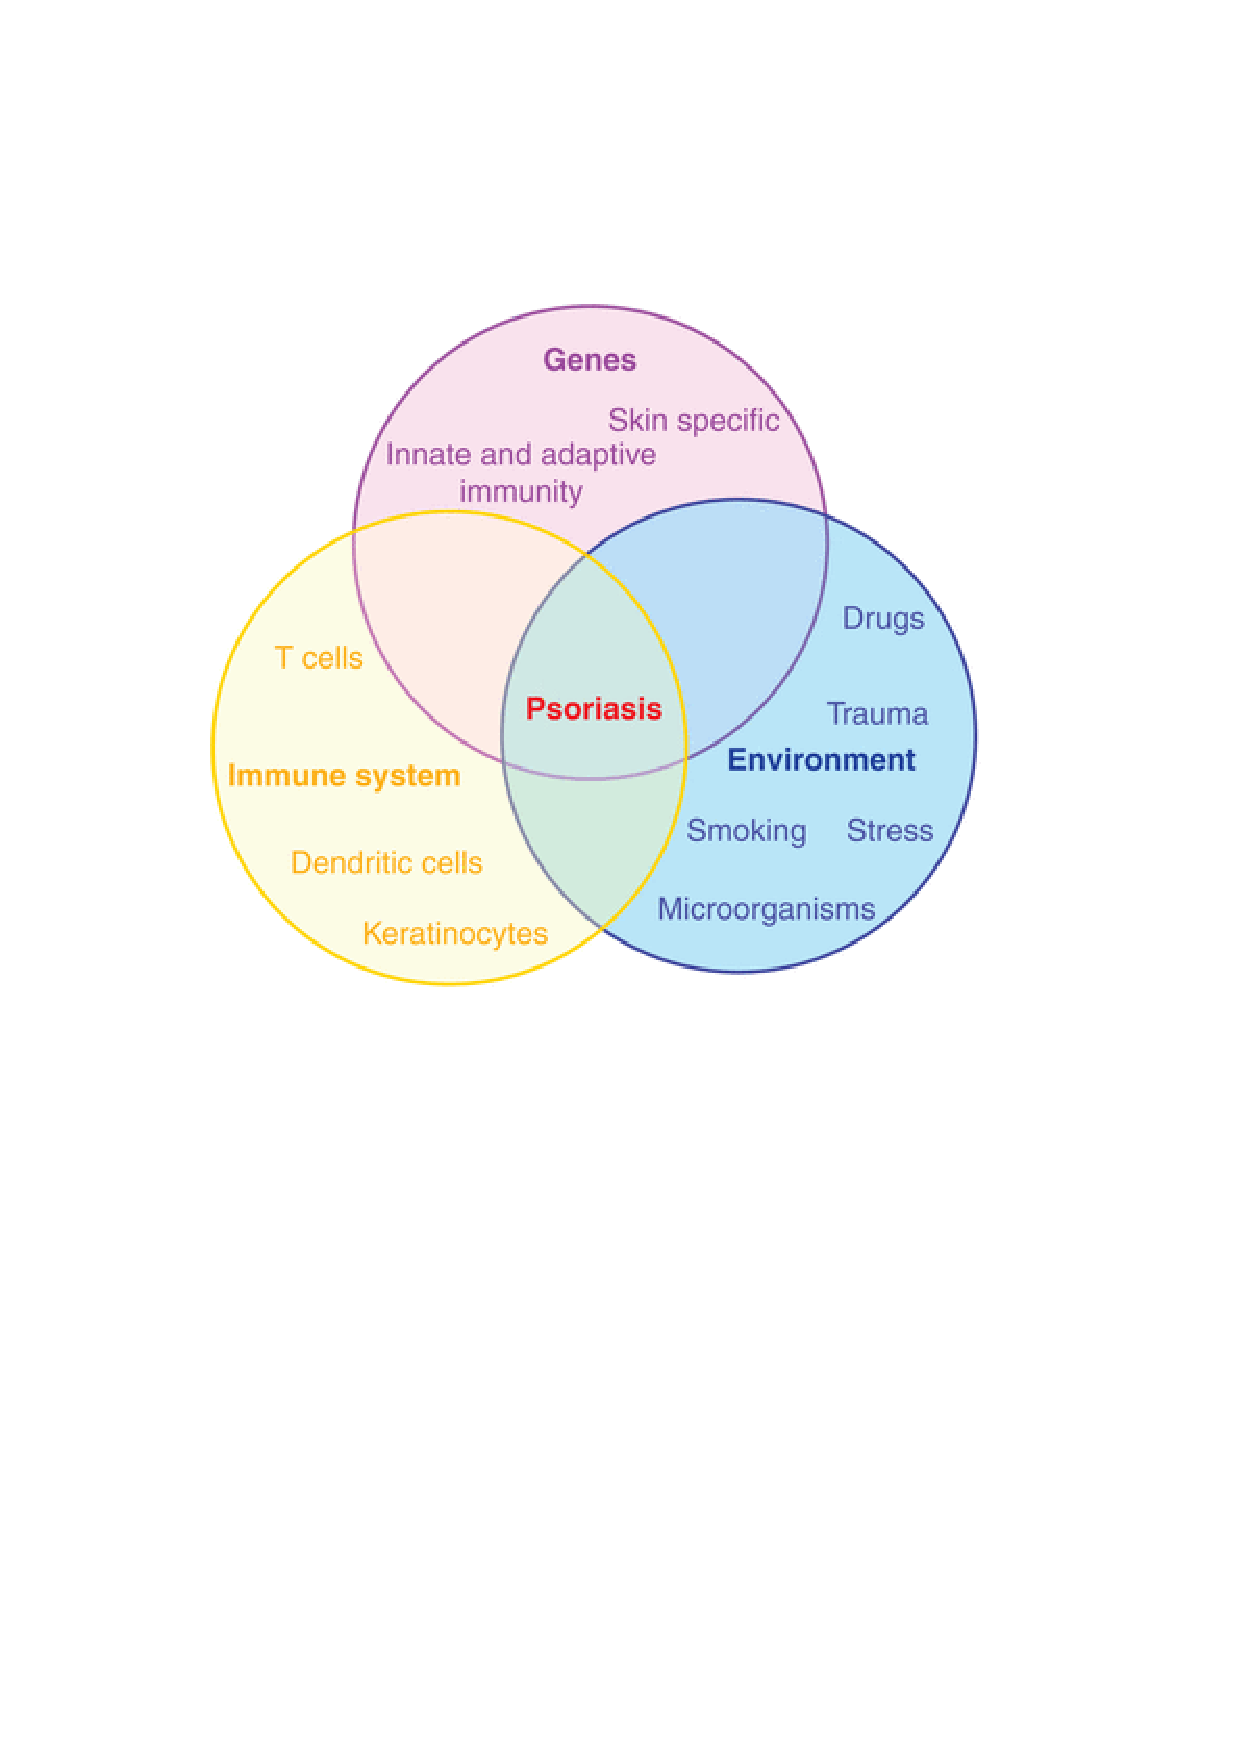
\includegraphics[width=\textwidth]{./Introduction/pdfs/PSO_aetiology_diagram_Di_Meglio_et_al_2014.pdf}
%\caption[Main factors involved in psoriasis disease aetiology]{\textbf{Figure adapted from \parencite{Meglio2014}}}
%\label{fig:PSO_aetiology_diagram}
%\end{figure}


\subsubsection{Histopathological alterations in skin and joints}

The epidermis is the most external structure of the skin and it is formed by approximately 90\% keratinocytes (KC) organised in a layer structure that self-renews in a time dependent manner from the bottom to the surface \parencite{Wikramanayake2014}. As the KC differentiate they undergo changes in morphology, replication ability and keratin composition of their intracellular matrix. In the context of psoriasis impaired epidermis cell renewal leads histological alterations and development of the psoriatic lesions. KC undergo upregulation in the proliferation rate (hyperplasia) that causes aberrant cell differentiation (parakeratosis) (ref) thickening of the epidermis and the subsequent scale formation (ref). Concomitantly, inflammation causes immune cell infiltration and hypervascularisation of the lesion driven by upregulation in the expression of angiogenic factors and activation of the endothelium \parencite{Perera2012}. 

In PsA, joint affection usually follows skin lesions and it involves a wide range of histological changes in the joints, particularly bone remodeling \parencite{Haddad2013}. One of the most common structural changes is the arthritis caused by the swelling and inflammation of the joints \parencite{Schett2011}. As result of this inflammation, alterations in bone remodeling leads to osteolysis with subsequent bone resorption and erosion at the affected joints \parencite{Mensah2017}. This phenomenon is particularly relevant in arthritis mutilans or chronic absortive arthritis, one of the most severe forms of PsA \parencite{Haddad2013}. Bone erosion is also the main histopathological process driving dactylatis, where bone lysis resolves in shortening of the digits \parencite{Gladman2005}. On the other hand, 35\% of the PsA patients undergo inflammation of the connective tissue at the insertion of tendons or ligaments, phenomenon known as enthesitis \parencite{McGonagle2011,Polachek2017}. Overtime, this causes debilitating structural changes due to formation of bony spurs along the insertion sites\parencite{Schett2011}.


\subsubsection{Dysregulation of the innate and adaptive immune response}
%link to the histological changes
The dysregulated  immune response in psoriasis and PSA is the result of the interaction between innate and adaptive immune cells (ref section) resulting in feedback loops involving a complex cytokine milieu. Among the most relevant cytokines of the innate immunity involved in disease initiation are IFN-$\alpha$ and IFN-$\gamma$ \parencite{Leanne2009}. They are mainly produced by circulating plasmacytoid DC (pDC) and myeloid DC (mDC), respectively, upon activation by KC proinflammatory cytokines \parencite{Perera2012}. Both are upregulated at the mRNA level in the lesional skin and contribute to lymphocyte recruitment and maintenance of DC activation \parencite{Schmid1994}. 

Another key cytokine in this dysregulated inflammatory response is TNF-$\alpha$ which has a prominent role in bone turnover and bone remodeling in PsA \parencite{Mensah2008}. It is produced by activated KC, mast cells but also by adaptive immune cells types, including infiltrated T helper(Th) 1 and Th17 cells infiltrated in the psoriatic lesion and PsA inflamed joints \parencite{Perera2012} and it induces activation of nuclear nactor kappa-light-chain-enhancer of activated B cells (NF-$\kapa$B) signaling pathways (ref). It also activates several kinase signaling pathways as well as cell death programs (ref). In the context of inflammation, NF-$\kapa$B represents a master transcriptional regulator of both, the innate and adaptive immune system that induces expression of proinflammatory cytokines, antiapoptotic genes and genes involved in chronic inflammation maintenance (ref). The importance of this transcription factor (TF) in psoriasis and PsA pathogenesis is reflected by the association with disease of several genetic variants in some of the negative regulators of its proinflammatory activity, including NF-$\kapa$B inhibitor alpha \textit{NFKBIA} and TNF receptor-associated factor 3 interacting protein 2 \textit{TRAF3IP2} (ref).
 
Interleukin-23 (IL23) and Th17 axis represents a key loop for the maintenance of psoriasis and PsA inflammatory response and a very important link between innate and adaptive immunity. IL-23 is an innate regulatory cytokine, mainly produced by mDC and macrophages homing the inflamed skin and it binds to the IL23 receptor (IL23R), which expression is upregulated in the DC and T cells of the lesion and in circulating Th cells (ref). In psoriasis, IL23 is the mediator for the pathogenic loop between activated KC and T cells (ref). Both IL-23 and IL-23R present protective and pathogenic genetic variants associated with psoriasis and PsA risk (ref). The activation of the IL-23 pathway leads importantly to increased IL17 production through NF-\kappaB activation by \textit{TRAF3IP2} (ref). IL17 favors maintenance of the adaptive immune mediated Th17 response through recruitment and activation of neutrophils, induction of proinflammatory cytokines including IL-1\beta and IL-6 and also perpetuation of KC activation (ref) (https://www.ncbi.nlm.nih.gov/pmc/articles/PMC3580541/). % add info
More recently, interleukin 22 (IL22) has arisen as another of the key cytokines in mediating the dysregulated cross talk between the innate and adaptive immune response. IL22 levels are increased in the psoriatic lesions and serum of patients and it is mainly produced by a subset of CD4$^+$ cells known as Th22 (ref). It mediates some of the histological changes in skin as well as AMP production by KC (ref).

% Maybe a paragraph to connect skin and joint affection Identical T cell clonality between skin and synovium https://ac.els-cdn.com/S0198885999000348/1-s2.0-S0198885999000348-main.pdf?_tid=5efa7316-fde5-11e7-8091-00000aacb360&acdnat=1516454913_dd20efb867f822d68d8b09873601e8ad

\subsubsection{Environmental factors and disease}

Several environmental triggers are known to be associated with increased risk and worsening of psoriasis and PsA development. A wide range of drugs including antidepressant, antihypertensive and anticytokine therapies have been clinically associated with initiation, exacerbation and worsening of psoriasis \parencite{Kim2010}. Infectious agents such streptococcal throat infection have likewise been associated with development of type I psoriasis \parencite{Gudjonsson2003,Valdimarsson2009, Diluvio2006}. Consistently with other chronic inflammatory disease such as IBD and AS, recent studies have also observed perturbation in the composition of the gut and skin microbiota in psoriasis and PsA patients. On the other hand, physical trauma, including tattoos, surgical incisions and mechanical stress can trigger the appearance of lesions in psoriatic uninvolved skin as well as joint inflammation in digits \parencite {Weiss2002,Nestle2009}. Lastly, as for most of the complex diseases, behavioral factors including smoking, alcohol and stress have been linked to psoriasis and PsA without a clear conclusion of their involvement in triggering disease \parencite{Meglio2014}.

\subsection{Cell types involved in psoriasis and PsA pathogenesis}
%Global report on psoriasis, 2016

Identifying the most relevant cell types contributing to psoriasis and PsA pathogenesis remains challenging. There has been a reinterpretation of both phenotypes that understands them as dynamic and continuous processes where different cell types became predominantly important at different stages of the pathology. 

KC are one of the most relevant cell type at early stages of psoriasis pathogenesis, which is reinforced by the genetic association between skin specific genes from the late cornified envelope (LCE) family and psoriasis \parencite{Tsoi2012}. Several studies have shown the role of KC as immune sentinels through MHC-II antigen presentation and production of antimicrobial peptides (AMP), cytokines and chemokines \parencite{Black2007}. There is evidence of complex formation between the cationic AMP LL-37 and self-DNA/RNA released by KC upon damaged triggered by environmental factors \parencite{Lande2007}. This complex acts as an antigen for activation of the skin-resident DC \parencite{Nestle2005} and that initiate and perpetuates the skin inflammatory response through secretion of pro-inflammatory cytokines, importantly IL-1, IL-6 and TNF-$\alpha$ \parencite{Feldmeyer2007, Arend2008, Nestle2009}. Studies in mouse models have also shown development of psoriatic lesions in immunodeficient mice upon human xenotransplant of psoriasis skin\parencite{Boyman2004}. Overall, these findings would support the hypothesis attributing the initiation of the chronic inflammatory response in psoriasis as the consequence of the epidermis dysfunction \parencyte{Proskch2008}. 

mDC and pDC are the professional APC also considered important innate immune cells in disease initiation through T cell activation and subsequent triggering of the adaptive immune response \parencite{Mahil20016}. %The relevance of antigen presentation in disease has been highlighted at the cellular \parencite{Rusell1972, Tiilikainen1980} and also at the genetic level with the psoriasis and PsA GWAS association of HLA-Cw*06:02 and ERAP1 \parencite{Strange2010}, which encodes for an aminopeptidase involved in the trimming of peptide antigens.
pDC are circulating cells absent in healthy skin that infiltrate into the lesional and uninvolved dermis of psoriatic lesions and get activated by the aforementioned KC self-DNA and LL-37 complex through Toll-like Receptor (TLR)-9 \parencite{Nestle2005, Lande2007}. In contrast, quiescent mDC are epidermal resident and upon secretion of IFN-$\alpha$ by pDC a 30-fold increase of mature mDC is observed in lesional skin but not in uninvolved or healthy tissue (ref). Different mDC subpopulation mediate the Th1 and Th17 response as well perpetuation of KC activation through IL-23 production (ref). Studies in immunodeficient psoriasis mice models have shown that blockage of downstream  IFN-$\alpha$ signaling or its production by pDC failed to induce T cell activation and onset of psoriasis \parencite{Nestle2005}. 

Neutrophils are also though to be closely involved in disease initiation through their ability to form neutrophil extracellular traps (NET)that contain host DNA and AMP, particularly LL-37 \parencite{Hu2016}. There is evidence of increased NET formation in peripheral blood and lesional skin of psoriasis patients and they seem to be contributing to pDC and CD4$^+$ T activation \parencite{Hu2016}. Neutrophils have also been identified in recent studies as one of the main sources of IL-17 production in the skin lesions \parencite{Lin2011} and they also release a wide range of proteases which some induce KC proliferation \parencite{Mahil2006}.

In the context of the innate immunity, the involvement of monocytes and macrophages in psoriasis and PsA has not been extensively studied. Resident macrophages in the healthy dermis undergo a 3-fold increase in lesional skin and they are involved in disease development through TNF$\alpha$ production \parencite{Perera2012, Mahil2016}. Different mice models for chronic psoriasiform skin inflammation have shown a key role of macrophage migration into the affected skin and TNF-$\alpha$ production for maintenance of the lesions \parencite{Stratis2006, Wang2006}. Some studies using psoriasis and PsA patients derived monocytes have also highlighted the systemic aspects of both pathologies. Psoriasis PBMC isolated monocytes have shown greater phagocytic and bactericidal activity compare to those from healthy individuals \parencite{Bar-Eli1979}. Later studies have also shown increased circulating intermediate monocytes (CD14$^{+}$ high CD16$^{+}$ high) and monocyte aggregation in psoriasis patients with subsequent enhanced platelet activation and angiogenesis \parencite {Golden2015}. %In PsA, synovial membranes levels of monocytes/macrophage metalloproteinases are comparable to those found in RA joints mediating bone erosion through differentiation of classical monocytes into osteoclasts \parencite{Hitchon2002}.

Historically, T lymphocytes have been considered one of the most relevant cell types in initiation and maintenance of psoriasis and PsA, and GWAS association with MHC-I also supports the role of T cells in disease. Report cases in humans have demonstrated that bone marrow transplantation can initiate or terminate psoriasis and, therefore, the role of bone marrow-derived T cells in disease pathophysiology \parencite{Eedy1990, Gardembas1990}. The percentage of circulating T cells in psoriasis has been reported to be dependent of severity. Different studies have shown reduced number of T cells in moderate-to-severe and severe psoriasis patients when compared to milder phenotypes and healthy controls. Despite this reduction, increased percentage of the memory populations CD4$^{+}$CD45RO$^{+}$ and CD8$^{+}$CD45RO$^{+}$ have been demonstrated in the same individuals\parencite{Lecewicz-Toruń2001,Langewouters2008}. There is still controversy regarding the total CD4$^+$ and CD8$^{+}$ abundance and CD4$^{+}$/CD8$^{+}$ ratios in PBMC, which may be due to the phenotype heterogeneity of psoriasis patients in the different studies \parencite{Lecewicz-Toruń2001,Cameron2003,Langewouters2008}. In PsA, no differences  abundance of circulatings T cells have been identified compared to healthy individuals \parencite{Costello1999}.

In healthy skin, CD4$^{+}$ and CD8$^{+}$ are found in the dermis and epidermis, respectively \parencite{Clark2006,Perera2012} and upon lesion development an increase in activated memory CD4$^{+}$CD45RO$^{+}$and CD8$^{+}$CD45RO$^{+}$ in the respective compartments can be detected as soon as 3 days after its appearance \parencite{Clark2006}, highlighting the importance of the memory population. \textit{In vivo} studies conducted in mice by Boyman and colleagues showed that development of psoriasis following engrafted human pre-lesional skin was dependent of local T cell proliferation and it did not required injection of additional factors \parencite{Boyle2013}. This supports the theory where recruitment of circulating T cells is restricted to the priming event and it is minimal afterward \parencite{Perera2012}. The relative importance of CD4$^{+}$versus CD8$^{+}$ in psoriasis initiation has been tested immunodeficient mice with pre-lesional skin xenografts followed with injection of purified activated T cell populations \parencite{Nickoloff1999}. These observations suggested a model where CD4$^{+}$ but not CD8$^{+}$ T cells where required for the progression of uninvolved to lesional skin in mice. Interestingly, injection of CD4$^{+}$ activated cells was followed by an increase in activated resident CD8$^{+}$ T cells expressing the acute activation marker CD69. It suggest a hypothesis where in the skin CD4$^{+}$ drive signaling for activation of resident T cells and the activated CD8$^{+}$ resident population are the main effector cells. In PsA, CD4$^{+}$ are significantly more abundant than CD8$^{+}$ cells in synovial tissues \parencite{Diani2015}. In contrast, CD8$^{+}$ expressing CD45RO are prevalent in the SF and they are also significantly increased when compared to controls \parencite{Costello1999}.

In addition to memory T cells, the contribution of regulatory T (Treg) cells have also been investigated to some extent due their role in immunosurveillance and self-tolerance in the context of autoimmune disease. Nevertheless, controversial results have been found regarding relative abundance and impaired function \parencite{Perera2012}. 

Based on the cytokine profile, psoriasis and PsA has been demonstrated to be a type 1 Th/Tc disease, where naive CD4$^{+}$ and CD8$^{+}$ cells get activated and proliferate in the presence of IL-12 and IFN-$\gamma$ \parencite{Austin1999,Perera2012}. Later studies also identified additional subsets including Th-17/Tc-17 and Th-22/Tc-22, which are mainly dependent on IL-23 and IL-6 for their activation, respectively \parencite{Mahil2016}. The importance Th17 cells and their IL-17 production has been assessed in skin, joints and blood, where increased IL-17 and also IL-23 mRNA and protein levels have been found in psoriasis and PsA patients compared to controls \parencite{Cai2012, reference for joints}. It has been shown that the predominant CD8$^{+}$ cells in the SF are  also IL-17 producers and their abundance correlates with markers of inflammation and structural changes in the joint \parencite{Menon2014}. This finding distinguishes PsA from other forms of arthritis such as RA and is in line with findings on skin that suggest a prominent role of CD8$^{+}$ IL-17 producing cells in the different stages of both pathologies. There is also evidence of the synergistic interaction between Th1 and Th17 cells which overall enhances the production of AMPs by KC \parencite{Kryczek2008}. Understanding of the importance of IL-17 has also led to the discovery of other immune cells producing this pivotal cytokine including innate immune lymphoid (ILC) cells and $\gamma$$\delta$ T cells which have also started to been investigated in the context of psoriasis and PsA pathophysiology and treatment \parencite{Meglio2014,Leijten2015}.
IL-17 producing cell have also been hypothesised to be responsible for the link between skin and joint lesions. Although the precise mechanisms for transition between psoriasis and PsA is unknown, studies using psoriasis and RA mice models have shown that skin lesions facilitate arthritis and joint inflammation % \parencite{}. 
It has been hypothesised that the presence of IL-17 producer cells in inflamed skin located nearby the enthesis of joint under physical stress could trigger the development of PsA.

\begin{figure}[H]
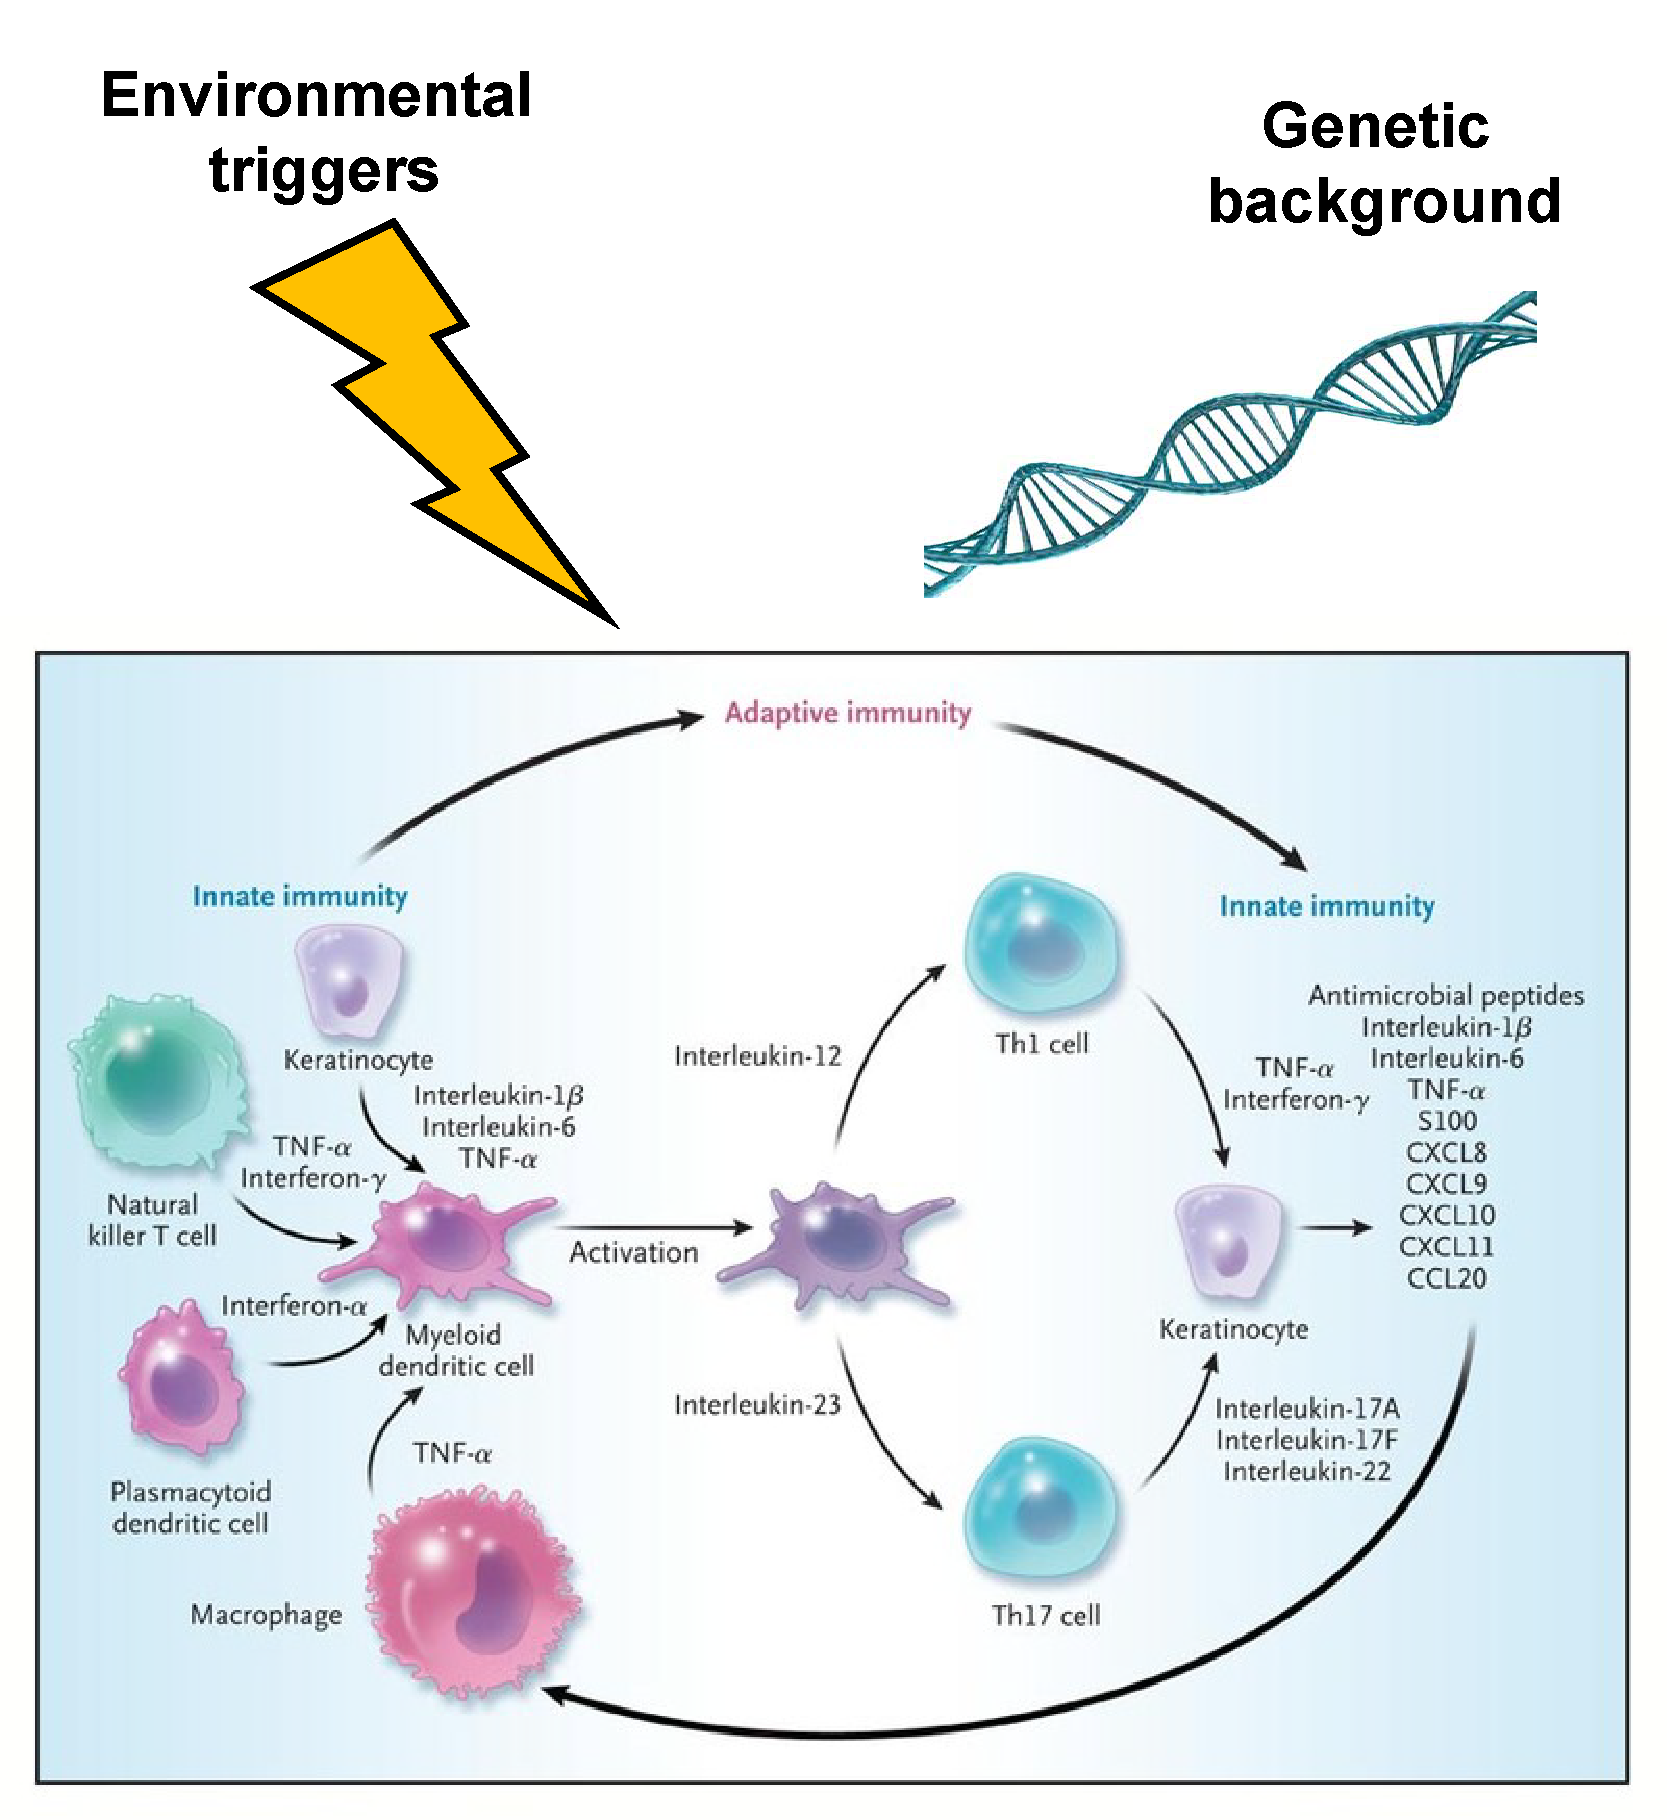
\includegraphics[width=\textwidth]{./Introduction/pdfs/PSO_adaptive_innate_immune_system_crosstalk.pdf}
\caption[Crosstalk between innate and adaptive immunity in psoriasis]{\textbf{Figure adapted from \parencite{Nestle2009}}}
\label{fig:PSO_immune_system_diagram}
\end{figure}

\subsection{Therapeutic intervention and prognosis}

Currently, there is no cure for either psoriasis or PsA and the different treatments available are focused in managing the disease manifestations and symptoms. The approach to treat them are usually dependent on the disease severity. Cases of mild-to-moderate psoriasis are usually managed with topical and systemic therapies \parencite{Menter2009}. Among the topical agents, corticosteroids and emollients are the most commonly used and affordable ones. Emollients are non-medicated agents that contribute to keep the skin soft and moist minimising the symptoms of itching and tenderness and they have been accepted as an adjunctive for the treatment of psoriasis. On the other hand, cortocosteroid in creams, shampoo and spray remain as the most widely spread medical topical treatment due to their antiinflammatory, antiproliferative, and immunosuppressive actions. Corticosteroids are classified based on the potency and they all exert their effect through binding to intracellular corticosteroid receptors and regulation of gene transcription \parencite{Tadicherla2009}. Although they are the most common way to treat mild forms of disease, some of them are approved only for short term treatments as side effects have been reported at a local and systemic level \parencite {Menter2009}. In the case of PsA presenting swelling of two or less joints intraarticular injection of glucocorticosteroids together with joint aspiration have shown to reduce pain and inflammation as a short-time measure \parencite{Coates2016}.    

For psoriasis, other topical treatments are used in combination with topical corticosteroids including ultra violet (UV) light therapy and vitamin D analogues, which inhibit KC proliferation, stimulate KC differentiation and inhibits T cell proliferation and other inflammatory mediators \parencite{Rizova2001}. Topical retinoids and calcineurin inhibitors are also used less frequently for the treatment of psoriasis and they have shown reduced systemic absorption and better suitability for long term treatments in some studies \parencite{Weinstein2003, Menter2009}.

Treatment of most forms of PsA and more moderate-to-severe psoriasis require the use of a broad range of systemic therapies. For mild cases of PsA with involvement of less than four joints and non radiological evidence of structural changes, nonsteroidal antiinflammatory drug (NSAID) are the most commonly used to help controlling the mild inflammatory symptoms and also helping to alleviate the pain and stiffness \parencite{Coates2016}. However, the use of NSAID is not recommended in patients presenting CVD comorbidities due to the increased risk associated with the use of these drugs \parencite{Bhala2013}. For those NSAID-resistant or more severe forms of PsA, disease-modifying antirheumatic drugs (DMARDs) including the an antagonist of folic acid methotrexate (MTX) and the phosphodiesterase 4 inhibitor apremilast have shown to immunosupressive effects on activated T cells and reduction of cytokine production, respectively \parencite{Schmitt2014, Gossec2016, Keating2017,Polachek2017}. However, increased risk of hepatotoxicity for the MTX \parencit{Menter2009} and gastrointestinal side effect  of apremilast \parencit{Menter2009} require requires ensuring appropriate dosing and surveillance. 


The use of biologic systemic agents tend to be the most specific but also expensive treatment for severe cases of psoriasis and PsA and they are not used as the first-line of treatment. These are molecular species generated in cell-based that modulate the immune response in a physiological based manner \parencite{Perera2012}. Among the biologic agents targeting cytokines, TNF$\alpha$ inhibitors (TNFi) have been broadly used for the past five decades to treat both, psoriasis and PsA since this is a pivotal cytokine in initiation and perpetuation of the inflammatory response. There are three TNFi approved for the treatment of psoriasis etanercept, infliximab and adalimumab \parencite{Ahil2016} and another two, certolizumab pegol and golimumab, also used in the management of PsA and other rehumatoid diseases  \parencite{Coates2016b}. All the TNFi are antibody-based agents but etanercep, that is a soluble receptor, and they also show differences in the frequency and via of administration as well as the efficacy, particularly in the specific improvement of skin or joint lesions \parencite{Mease2000}. Although TNF-$\alpha$ blockade is one of the most effective treatments some patients experience common side effects such as increased risk of infection, reactivation of latent infections, demyelinating disease and induced pustular psoriasis have been identified \parencite{Nickoloff2004}. Between 20 to 50\% of the patients fail to respond to the first TFNi and require switching to a second or third one \parencite{Abramson2016}. Lately, new biologic therapies have been developed to target other key cytokines in the pathogenesis of PsA and psoriasis, such as IL-12, IL-23 (ustekinumab) or  IL-17 (secukinumab and ixekizumab) \parencite{Mahil2016}. These new biologics represent a substantial benefit for treating patients and they are routenely administered to individuals failing to respond after a switch to a second TNFi \parencite{Coates2016b}.
 

indirect evidence mDC also produce interleukin 12 (IL12) that could contribute to IFN-$\gamma$ production in lesional skin and inflammed synovium (ref). 


\section{Genetics of psoriasis and psoriatic arthritis}

As complex diseases, the risk to develop psoriasis and PsA is not only influenced by the surrounding environmental conditions but also by the genetic background of each individual. Determining the magnitude of contribution of the genetic factors in the development of these disease and identifying the exact genes or regions involved in the predisposition to psoriasis and PsA remains challenging. 


\subsection{Heritability}

Several studies have shown a trend towrads the increase of psoriasis and PsA prevalence over the last 30 years in different countries \parencite{Organization2016}. This importantly reflects changes in life style habits and it highlights the need to better understand the genetic factors that predispose to disease upon interaction with environmental stresses.

The contribution of genetics in the development of psoriasis has also been demonstrated in several twins studies. The concordance of psoriasis has been shown to be greater in monozygotic (33-55\%) compared to dizyogtic (13-21\%) twins with some variation between studies and populations, estimating an 80\% of heritability in this condition \parencite{Faber1974, Duffy1993, Pendersen2008}. For PsA, similar concordance between mono- and di- zygotic twins has been shown, probably due to lack of statistical power and appropriate diagnosis \parencite{Pendersen2008}. In the general population, approximately 40\% of the patients with psoriasis or PsA have family history in first degree relatives \parencite{Gladman1986}. Interestingly, the recurrence in first-degree relatives ha been shown to be greater in PsA (40) compared to psoriasis (8) in a study in Icelandic population \parencite{Chandran2009}. This could suggest differences in the heritability between the two phenotypes and maybe an stronger genetic contribution in PsA.

\subsection{Genetic studies}
Different approaches have been undertaken to uncover the genetic variability contributing to the predisposition to psoriasis and PsA. The appearance of next generation sequencing (NGS) techniques and the progressive reduction of cost has allowed to move from candidate genes studies looking at the genetic variability at particular locus to a genome-wide approach.

\subsubsection{Non-GWAS and linkage studies}
The study of psoriasis and PsA genetics architecture started with linkage analysis in family pedigrees with autosomal dominant condition to try to . The use of this approach yielded nine psoriasis susceptibility loci (PSORS1-9) \parencite{Capon2017} with the strongest association in PSORS1 \parencite{International2003}. PSORS1 lies within chromosome 6p21.3 and its identification by linkage analysis confirmed the association previously identified in serological studies between psoriasis susceptibility and the MHC I \parencite{Rusell1972, Tiilikainen1980}. Importantly, Mendelian forms of disease with rare highly penetrant mutations have been identified in family studies for two genes within PSORS2 (17q25): zinc finger protein 750 (\textit{ZNF750}) \parencite{Tomfohrde1994} and caspase domain family member 14 (\textit{CARD14}) \parencite{Jordan2012}. Rare gain of function and \textit{de novo} mutations and also common variants in \textit{CARD14} have been identified in psoriasis and PsA patients, suggesting an important role of the genetic variation in this gene for Mendelian and multifactorial forms of both \parencite {Jordan2012, GWAS study}. In PsA, a region close to the psoriasis PSORS8 was also identified \parencite{Karason2003}. Nevertheless, the ability of independent studies to only reproduce PSOR1, 2 and 4, highlighted the limitations of the linkage studies to understand the genetics of complex diseases \parencite{Capon2017}. Gene based studies in psoriasis and PsA have also identified the relevance of genetic variability in the activating killer immunoglobulin receptors 2DS1 (KIR2DS1) \parencite{Łuszczek2004, Williams2005}, similarly to AS and RA \parencite{Carter2007, Yen2001}. This receptor is expressed on NK and NK T cells and mainly triggered by HLA-Cw*06:02. Similarly, specific association with PsA but not psoriasis was found for microsatellites and promoter polymorphisms in TNF-$\alpha$ \parencite{H\"{o}hler2002}. 



\subsubsection{Genome-wide association studies}
The technological advances experienced in sequencing and genotyping has allowed to implement association studies at a genome-wide scale. The genome-wide association studies (GWAS) have benefit from the understanding of common (frequency ${>}$1\%) single base-pair changes know as single nucleotide polimorphisms (SNPs) in different populations through whole genome sequencing (WGS) projects such as HapMap \parencite{The international HapMaP Consortium} project and the 1000 Genomes project \parencite{The 1000 Genomes}. GWAS have focused in the association to a particular phenotype of single-nucleotide bi-allelic substitutions with minor allele frequency ${>}$5\% in a case-control design \parencite{Ku2010}. This followed the hypothesis driving the field of complex diseases where common diseases are more likely to be caused by common variants \parencite{Schork2009}. Due to the organisation of the genome into segments of strong linkage desiquilibrium (LD) where genetic variants are strongly correlated with each other, the genotyped SNPs in GWAS are used a proxy for the disease causative variant. Disease causal variants can be non-genotyped SNPs or other type of genetic variability such as copy number variants (CNVs), also highly frequent in the genome \parencite{Hirschhorn2005, Ku2010}. In the context of complex diseases, GWAS have greater power than the previous linkage studies when looking at the influence of many loci with low penetrance and small effects in disease risk \parencite{Cui2010}.

%-What they are about: type of variation that they take into account
%-Advantages versus previous approaches

Since the improvement of genotyping technologies several GWAS studies have been performed in psoriasis and PsA (Table). Some of them have included individuals affected with psoriasis and PsA indistinctly, whereas others have performed stratification within the same study \parencite{Ellinghaus2010, Ellinghaus2012}.Most of the studies have been performed in Caucasian European or North American cohorts but lately few GWAS studies Chinese populations have also been published \parencite{Zhang2009, Sun2010, Yin2015}. The earlier studies were performed in discrete cohort sizes with moderate power that confirmed association with loci overlapping the PSOR1, PSOR2 and PSOR4 regions from the linkage studies. HLA-C was identified as the most significant locus with the greatest effect size which account for approximately 50\% of psoriasis heritability.  
Since the first psoriasis GWAS analysis in 2007 more the number of risk loci associated with psoriasis and psA have increased -Main studies in psoriasis and PsA: limitations of the phenotypes and different populations




-Possibility of transethnic studies
Mention the GWAS in Asian populations

-Low frequency and rare variants

-Exome GWAS
	Dand 2017
	
-Introduction to the limitations of GWAS including INDEL and inversion that may be covering an important part of the heritability
	Missing heritability
	Critical paper about GWAS in general
	Bias towards common SNps
	Need of a better understanding of the LD between different type of variation to design appropriate genotyping arrays with SNPs being appropriate surrohgate markers of genetic variation
	Talk about Andy/Ola project with nanopore...
	
\subsection{MHC and non-MHC associations with disease risk}
Based on reading the GWAS papers (summary)

\subsection{The role of coding and non-coding variants in disease susceptibility}
More generale and examples in psoriasis and PsA

\subsection{The role of GWAS studies in highlighting disease relevant tissues}
Indicate main pathways highlighted by the GWAS studies and also some pathways analysis studies
Shared susceptibility loci e.g Ellinghaus et al., 2012


%\subsection{GWAS and functional genomics of psoriasis and other complex diseases}
%\textbf{HLA-C*06:02 mediated pathogenesis}
%The association of the allele HLA-C*06:02 with PSO was first established through serological studies \parencite{Rusell1972, Tiilikainen1980} and it was later on confirmed the association of the region through genetic studies (Ellinghaus et al., 2010; Strange et al., 2010; Stuart et al., 2010; Sun et al., 2010)
%
%the  identification of the precise gene within the associated region of the genome is challenging. Although some earlier studies using microsatellites as markers excluded HLA-C, later genetic studies using dense genotyping that allows better haplotype definition have confirmed HLA-C*06:02 as the susceptibility allele and have identified a single nucleotide polymorphism (SNP) within the gene to drive the greatest association  to disease \parencite{Nair2006, Nair2009} showing 10-fold increase of PSO risk in homozygosis \parencite{Perera2012}
%
%
%number of HLA-C alleles 2375 encoding for 1677 proteins \parencite{Robinson2013}. Particularly, HLA-Cw*06 has 51 different subtypes 
%Regarding allele frequency it changes among ethnic populations. 5553 British Caucasian individuals from the OBB HLA-C allele of greater frequency was HLA-C*07:01 (High resolution HLA haplotyping by imputation for a British population bioresource Neville2017)
%
%
%
%Association of HLAC with other diseases such as Hepatitis C, PsA, primary sclerosing cholangitis and Grave´s disease \parencite{Blais2011}
%
%However, the detailed role of HLA-C*06:02 in the pathogenesis of PSO remains uncertain partly due to the homology between different MHC-In and the polymorphic nature of HLA-C. 
	%Presence of SNPs in minimal promoter and enhancer region that affects expression levels of HLA-C alleles \parencite{Clop2013, Hundhausen2012}. However HLA-Cw*0602 transcript levels do not differ significantly between normal and psoriatic showing responsiveness to proinflammatory cytokines and suggesting the association is not explained by alteration in regulation of gene expression \parencite{Hundhausen2012}. 
	%Lack of functional studies showing specific antigen or interacting proteins recognised by this allele
	%
%HLA-C is  is a heterodimer consisting of a heavy chain and a light chain and expressed in the surface of most of the cells, including antigen presenting cells (APC); however it has lower expression levels and degree of polymorphism than HLA-A and HLA-B ( Low HLA-C expression at cell surfaces correlates with increased turnover of heavy chain mRNA).
%
 %The major role of HLA-C has been assumed to be in acting as a ligand for killer immunoglobulin receptors (KIRs) expressed on natural killer (NK) cells however it is also recognised by TCR of CD8+ cells, not being clear if it exerts its pathogenic role through T cell or NK regulation 
%APC can activate immune response through presentation of processed antigens to CD8+ T cells, very abundant in the lesional epidermis due to inflitration that antigen could be T cell recognition of self-peptides hypothesis reinforced by epistasia with ERAP1 \parencite{Strange2010}, which encodes for an aminopeptidase involved in the trimming of peptide antigens. ERAP1  locus  is  only  associated  with  PSO  in  individuals carrying the HLA-C risk allele. The presentation of autoantigens(Although there are some studies regarding the self-tolerance and presence of autoantigenes as disease trigger \parencite{Lande2007}, the autoimmune aetiology of PSO is still under debate) to CD8+ T cells that clonally expand in psoriasis lesions has been reinforced by the observation of melanocytes as skin-specific target cells of an HLA-C*06:02-restricted psoriatic T cell response. We found that a CD8+ TCR, which we had reconstituted from an epidermal CD8$^+$ T cell clone of an HLA-C*06:02-positive psoriasis patient specifically recognises HLA-C*06:02-positive melanocytes. we observed numerous CD8$^+$ T cells in psoriasis lesions attacking melanocytes, the only epidermal cells expressing ADAMTSL5. Furthermore, ADAMTSL5 stimulation induced the psoriasis signature cytokine, IL-17A %reinfoce 
%, in CD8$^+$ T cells from psoriasis patients only, supporting a role as psoriatic autoantigen. % fact that CD4 are not reactive to autoantigen and that they are the first infiltrated cell type
%This unbiased analysis of a TCR obtained directly from tissue-infiltrating CD8$^+$ T cells reveals that in psoriasis HLA-C*06:02 directs an autoimmune response against melanocytes through autoantigen presentation. We propose that HLA-C*06:02 may predispose to psoriasis via this newly identified autoimmune pathway \parencite{Arakawa2015}.
%
%HLA-Cw*06:02 can be recognised by the inhibitory receptor KIR2DL1 and the activatory receptor KIR2DS1.  Some studies have shown KIR2DS1 was present in 85\% of the patients but only in 51\% of the controls
%NK cells are important regulators of immune responses \parencite{Luszczek2004}. Their function extends beyond killing of infected or transformed cells. Interactions with dendritic cells, macrophages, and fetal trophoblast cells can regulate NK cell activity by influencing cytokine production, cytotoxicity and stimulation of T helper-1 responses. 
%
%
%A similar inflammatory skin phenotype, which was also shown to be T-cell-dependent (Breban et al., 1996), was seen in rats transgenically expressing high levels of HLA-B27 and human β2-microglobulin (Tg(HLA-B*2705, B2M)33-3Trg; Table S1). However, these animals also developed multisystem inflammatory disease characterized by arthritis and colitis (Hammer et al., 1990).
%
%
%
 %
%
   %
%
%
%
%
%Nevertheless, other studies have demonstrated development of PSO in wild type mice upon bone marrow transplantation from mice with PSO-like phenotype
%
%
%
%
%
%
%\subsubsection*{Epigenetics and gene expression}
%\textbf{Understanding the chromatin landscape}
%\textbf{Chromatin accessibility}
%\textbf{Histones modifications}
%\textbf{Understanding the chromatin landscape}
%\textbf{Transcription factor occupancy}
%\textbf{Chromatin interaction}
%
%
%% For later when talking about cohort Approximately one third of patients have moderate to severe disease, which affects more than 10 % of body surface area, and usually necessitates systemic medications.